\subsection{Versão 1 - Início do sistema de Cotas, Lei Nº 12.711 de 2012}
\label{versao1}

Inicialmente o sistema de ingresso foi construído sem considerar cotas, ou seja, a classificação era por pontuação ou nota de vestibular, não havia exigência de lei em função de reserva de vagas. As chamadas para matrículas eram realizadas pela ordem geral de classificação e alguns critérios de desempate. Hoje apenas alguns tipos de processos seguem este molde, como por exemplo cursos de curta duração, ou cursos internos que não se aplicam à legislação.

Com o surgimento da lei Nº 12.711/2012 vem também a demanda do governo para que as instituições reservem 50\% das vagas para estudantes do ensino médio exclusivamente em escolas públicas, e dentro destes 50\% deveria ser reservado um percentual para estudantes cuja renda familiar fosse inferior a 1.5 salários mínimos per capita:

\begin{citacao}
Parágrafo único.  No preenchimento das vagas de que trata o caput deste artigo, 50\% (cinquenta por cento) deverão ser reservados aos estudantes oriundos de famílias com renda igual ou inferior a 1,5 salário-mínimo (um salário-mínimo e meio) per capita.

Art. 3o  Em cada instituição federal de ensino superior, as vagas de que trata o art. 1o desta Lei serão preenchidas, por curso e turno, por autodeclarados pretos, pardos e indígenas, em proporção no mínimo igual à de pretos, pardos e indígenas na população da unidade da Federação onde está instalada a instituição, segundo o último censo do Instituto Brasileiro de Geografia e Estatística (IBGE) \cite{leicotas}.
\end{citacao}

Com este objetivo o algoritmo de classificação que era uma consulta SQL foi separado em 3 funções PHP de nome: \textit{calcula\_vagasAcoesAfirmativas}, \textit{aprova\_Candidatos} e \textit{retorna\_OrdemdePreenchimentodeVagasNaoOcupadas}.  A primeira com função de gerar o quadro de vagas, a segunda a seleção dos candidatos para serem aprovados e atualizar a contagem de vagas em cada categoria e a ultima para retornar a ordem de preenchimento em caso de sobra de vagas.

Tendo em vista que há uma divisão categórica das vagas entre os candidatos, foi preciso criar 5 tipos de situações de classificação para cada combinação de cotas possível, essas categorias foram definidas conforme o Quadro \ref{quadro_categoriasv1}.

\begin{quadro}
\caption{Lista de categorias de cotas da versão 1}
\label{quadro_categoriasv1}
\centering
\begin{tabular}{ l l }
   \cline{1-1}\cline{2-2}  
    \multicolumn{1}{|p{5.850cm}|}{\textbf{CLAG}} &
    \multicolumn{1}{p{8.217cm}|}{Ampla concorrência ou classificação geral 
( todos os candidatos concorrem )}
  \\ 
   \cline{1-1}\cline{2-2}  
    \multicolumn{1}{|p{5.850cm}|}{\textbf{EPRIPPI}} &
    \multicolumn{1}{p{8.217cm}|}{Candidatos que estudaram em Escola Pública com Renda Inferior a 1.5 salários mínimos per capita e autodeclarados Pretos, Pardos ou Indígenas}
  \\    
   \cline{1-1}\cline{2-2}  
    \multicolumn{1}{|p{5.850cm}|}{\textbf{EPRINPPI}} &
    \multicolumn{1}{p{8.217cm}|}{Candidatos que estudaram em Escola Pública com Renda Inferior a 1.5 salários mínimos per capita NÃO são autodeclarados Pretos, Pardos ou Indígenas; }
  \\    
   \cline{1-1}\cline{2-2}  
    \multicolumn{1}{|p{5.850cm}|}{\textbf{EPRSPPI}} &
    \multicolumn{1}{p{8.217cm}|}{Candidatos que estudaram em Escola Pública com Renda Superior a 1.5 salários mínimos per capita e autodeclarados Pretos, Pardos ou Indígenas}
  \\     
   \cline{1-1}\cline{2-2}  
    \multicolumn{1}{|p{5.850cm}|}{\textbf{EPRSNPPI}} &
    \multicolumn{1}{p{8.217cm}|}{Candidatos que estudaram em Escola Pública com Renda Superior a 1.5 salários mínimos per capita NÃO são autodeclarados Pretos, Pardos ou Indígenas}
  \\       
  \hline

 \end{tabular} 
\end{quadro}


\newpage
Dadas as situações de classificação possíveis o primeiro passo do algoritmo é gerar um quadro de vagas para cada tipo de cota, tendo como base o percentual do \gls{IBGE} e o total de vagas para o curso. O trecho de código desenvolvido será apresentado no Código Fonte \ref{lst:quadrovagas}.


\lstinputlisting[language=PHP, 
caption=Função que calcula o quadro de vagas
,label=lst:quadrovagas]{chapters/trechos_codigo/calculaquadrovagas.m}

Basicamente o que a função \textit{calcula\_vagasAcoesAfirmativas} faz é separar as vagas o seguinte passo a passo:

\begin{enumerate}
    \item Dado o total de vagas do curso;
    \item Obter o percentual de escola pública;
    \item Obter o percentual de proporção de PPI do IBGE no estado de oferta;
    \item Multiplicar o total de vagas pelo percentual de Escola Pública (50\%) e armazenar o valor em AAEP;
    \item Obter o total reservado para ampla concorrência (CLAG), diminuindo o total de vagas pelo reservado ao sistema de cotas AAEP;
    \item Dividir o total de vagas AAEP em 50\% para candidatos de Renda Inferior a 1.5 (AAEPRI) e 50\% para candidatos de Renda Superior a 1.5 (AAEPRS);
    \item Dentro do total de vagas AAEPRI, deve-se calcular a proporção reservada pelo IBGE para cotistas PPI (Preto, Pardo, Indígenas) que também possuam Renda Inferior a 1.5 salários mínimos e armazenar em AAEPRIPPI;
    \item O total de vagas de estudantes de Renda Inferior que NÃO são autodeclarados PPI (AAEPRINPPI) é obtido após diminuir o total de vagas para renda inferior AAEPRI - o total armazenado em (AAEPRIPPI).
    \item Dentro do total de vagas AAEPRS, deve-se calcular a proporção reservada pelo IBGE para cotistas PPI (Preto, Pardo, Indígenas) que também possuam Renda Superior a 1.5 salários mínimos e armazenar em AAEPRSPPI;
    \item O total de vagas de estudantes de Renda Superior que NÃO são autodeclarados PPI (AAEPRSNPPI) é obtido após diminuir o total de vagas para renda inferior AAEPSI - o total armazenado em (AAEPRSPPI).
\end{enumerate}{}

Um exemplo do resultado da geração do quadro de vagas, para um cenário de curso com 40 vagas,  pode ser visto na Figura \ref{fig:cenario1}.

\begin{figure}[ht!]
\centering

\caption{\textmd{Cenário de distribuição versão 1}}
\label{fig:cenario1}
\fcolorbox{gray}{white}{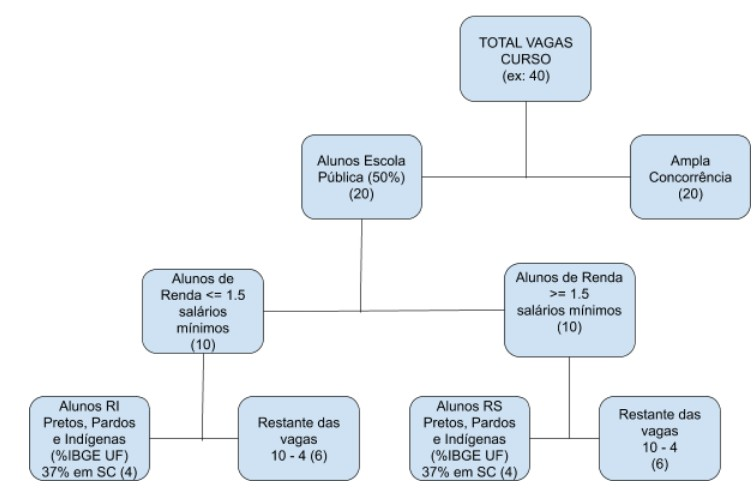
\includegraphics[width=0.67\textwidth]{chapters/sistemaingresso_versoes/cenarios/cenario1.jpg}}

\par\medskip\textbf{Fonte:} Elaborada pelo autor (2019). \par\medskip
\end{figure}



\newpage
Tendo com base o quadro de vagas o algoritmo de classificação de candidatos utiliza a função \textit{aprova\_Candidatos} descrita no Código Fonte \ref{lst:algoritmoaprovacao}, fazendo a seleção dos candidatos para aprovação em cada categoria até atingir o total de vagas disponível. 

\lstinputlisting[language=PHP, 
caption=Função de aprovação de candidatos
,label=lst:algoritmoaprovacao]{chapters/trechos_codigo/aprovacandidatos.m}

Por fim, o algoritmo utiliza a função \textit{retorna\_OrdemdePreenchimentodeVagasNaoOcupadas} obter a prioridade por lei quando sobra vaga de uma determinada categoria de cota, por motivo de falta de candidatos inscritos (Código Fonte \ref{lst:sobravagas}).

\lstinputlisting[language=PHP, 
caption=Função de prioridade em caso de sobra de vagas
,label=lst:sobravagas]{chapters/trechos_codigo/sobravagas.m}

Após análise no controle de versão pode-se identificar que as funções eram utilizadas em diferentes etapas e tipos de processo do sistema. No entanto a equipe que desenvolveu o sistema não teve preocupação na organização do código e fez a cópia em vários pontos do sistema, trazendo ainda mais problemas de manutenção no sistema. Os arquivos envolvidos, assim como os dados do controle de versão serão listados nas Tabelas \ref{tabela_arquivosv1_1}, \ref{tabela_arquivosv1_2}, \ref{tabela_arquivosv1_3} e \ref{tabela_arquivosv1_4}.

\begin{table}[ht!]
\centering
\caption{Versionamento do arquivo corrigir.php}
\label{tabela_arquivosv1_1}
\resizebox{\textwidth}{!}{
\begin{tabular}{@{}|l|l|@{}}
\toprule
\multicolumn{2}{|c|}{ingresso/admin/admin/correcao/corrigir.php}                                        \\ \midrule
\textbf{Total de linhas de código}                               & 1129                                 \\ \midrule
\textbf{Total de funções utilizadas}                             & 267 funções (incluídas e importadas) \\ \midrule
\textbf{Total de funções / algoritmo de cotas}                   & 5 funções                            \\ \midrule
\textbf{Número de linhas envolvidas / algoritmo de cotas}        &                                      \begin{tabular}{@{}|l|l|@{}}
\toprule
\textbf{processar\_Correcao}                             & 96 linhas de código \\ \midrule
\textbf{calcula\_vagasAcoesAfirmativas}                  & 33 linhas de código \\ \midrule
\textbf{aprova\_Candidatos}                              & 73 linhas de código \\ \midrule
\textbf{retorna\_OrdemdePreenchimentodeVagasNaoOcupadas} & 27 linhas de código \\ \midrule
\textbf{alimenta\_Classificacao}                         & 35 linhas de código \\ \bottomrule
\end{tabular}
    \\ \midrule
\textbf{Commits relevantes}                         & 31 commits desde  11/02/2015         \\ \midrule
\textbf{Número de programadores envolvidos nos commits}          & 2                                    \\ \midrule
\textbf{Total de linhas de código para a implementação de cotas} & 264 linhas                           \\ \bottomrule

\end{tabular}}

\par\medskip\textbf{Fonte:} Elaborada pelo autor (2019). \par\medskip

\end{table}

\begin{table}[ht!]
\centering
\caption{Versionamento do arquivo informar\_classificacao01\_sorteio.php}
\label{tabela_arquivosv1_2}
\resizebox{\textwidth}{!}{
\begin{tabular}{@{}|l|l|@{}}
\toprule
\multicolumn{2}{|c|}{ingresso/admin/admin/semprova/informar\_classificacao01\_sorteio.php}                                        \\ \midrule
\textbf{Total de linhas de código}                               & 1360                                 \\ \midrule
\textbf{Total de funções utilizadas}                             & 236 funções (incluídas e importadas) \\ \midrule
\textbf{Total de funções / algoritmo de cotas}                   & 5 funções                            \\ \midrule
\textbf{Commits relevantes}                         & 61 commits desde  11/02/2015         \\ \midrule
\textbf{Número de programadores envolvidos nos commits}          & 2                                    \\ \bottomrule
\end{tabular}}

\par\medskip\textbf{Fonte:} Elaborada pelo autor (2019). \par\medskip
\end{table}

\begin{table}[ht!]
\centering
\caption{Versionamento do arquivo informar\_classificacao01.php}
\label{tabela_arquivosv1_3}
\resizebox{\textwidth}{!}{
\begin{tabular}{@{}|l|l|@{}}
\toprule
\multicolumn{2}{|c|}{ingresso/admin/admin/semprova/informar\_classificacao01.php}                                        \\ \midrule
\textbf{Total de linhas de código}                               & 1162                                 \\ \midrule
\textbf{Total de funções utilizadas}                             & 88 funções (incluídas e importadas) \\ \midrule
\textbf{Total de funções / algoritmo de cotas}                   & 6 funções                            \\ \midrule
\textbf{Commits relevantes}                         & 14 commits desde  11/02/2015         \\ \midrule
\textbf{Número de programadores envolvidos nos commits}          & 2                                    \\ \bottomrule
\end{tabular}}
\par\medskip\textbf{Fonte:} Elaborada pelo autor (2019). \par\medskip
\end{table}

\begin{table}[ht!]
\centering
\caption{Versionamento do arquivo  semprova/classificacao01\_sorteio.php}
\label{tabela_arquivosv1_4}
\resizebox{\textwidth}{!}{
\begin{tabular}{@{}|l|l|@{}}
\toprule
\multicolumn{2}{|c|}{ingresso/admin/admin/semprova/informar\_classificacao01\_sorteio.php}                                        \\ \midrule
\textbf{Total de linhas de código}                               & 1363                                 \\ \midrule
\textbf{Total de funções utilizadas}                             & 119 funções (incluídas e importadas) \\ \midrule
\textbf{Total de funções / algoritmo de cotas}                   & 6 funções                            \\ \midrule
\textbf{Commits relevantes}                         & 24 commits desde  11/02/2015         \\ \midrule
\textbf{Número de programadores envolvidos nos commits}          & 3                                    \\ \bottomrule
\end{tabular}}
\par\medskip\textbf{Fonte:} Elaborada pelo autor (2019). \par\medskip
\end{table}


Com base nesse levantamento pode-se observar uma quantidade considerável de código fonte envolvido para desenvolvimento de regras para classificação de candidatos. Como tentativa de dar celeridade no processo de desenvolvimento de correções e na criação de futuras versões, os problemas de código duplicado foram reduzidos por meio de refatoração nas versões posteriores do algoritmo de classificação. Na Seção \ref{versao2} são apresentados os dados sobre o controle de versão, pós refatoração realizada em função de novas demandas de alteração da legislação.
